%%%%%%%%%%%%%%%%%%%%%%%%%%%%%%%%%%%%%%%%%
% Beamer Presentation
% LaTeX Template
% Version 1.0 (10/11/12)
%
% This template has been downloaded from:
% http://www.LaTeXTemplates.com
%
% License:
% CC BY-NC-SA 3.0 (http://creativecommons.org/licenses/by-nc-sa/3.0/)
%
%%%%%%%%%%%%%%%%%%%%%%%%%%%%%%%%%%%%%%%%%

%----------------------------------------------------------------------------------------
%	PACKAGES AND THEMES
%----------------------------------------------------------------------------------------

\documentclass{beamer}

\mode<presentation> {

% The Beamer class comes with a number of default slide themes
% which change the colors and layouts of slides. Below this is a list
% of all the themes, uncomment each in turn to see what they look like.

%\usetheme{default}
%\usetheme{AnnArbor}
%\usetheme{Antibes}
%\usetheme{Bergen}
%\usetheme{Berkeley}
%\usetheme{Berlin}
%\usetheme{Boadilla}
%\usetheme{CambridgeUS}
%\usetheme{Copenhagen}
%\usetheme{Darmstadt}
%\usetheme{Dresden}
%\usetheme{Frankfurt}
%\usetheme{Goettingen}
%\usetheme{Hannover}
%\usetheme{Ilmenau}
%\usetheme{JuanLesPins}
%\usetheme{Luebeck}
%\usetheme{Madrid}
%\usetheme{Malmoe}
%\usetheme{Marburg}
%\usetheme{Montpellier}
%\usetheme{PaloAlto}
%\usetheme{Pittsburgh}
\usetheme{Rochester}
%\usetheme{Singapore}
%\usetheme{Szeged}
%\usetheme{Warsaw}

% As well as themes, the Beamer class has a number of color themes
% for any slide theme. Uncomment each of these in turn to see how it
% changes the colors of your current slide theme.

%\usecolortheme{albatross}
%\usecolortheme{beaver}
\usecolortheme{beetle}
%\usecolortheme{crane}
%\usecolortheme{dolphin}
%\usecolortheme{dove}
%\usecolortheme{fly}
%\usecolortheme{lily}
%\usecolortheme{orchid}
%\usecolortheme{rose}
%\usecolortheme{seagull}
%\usecolortheme{seahorse}
%\usecolortheme{whale}
%\usecolortheme{wolverine}

%\setbeamertemplate{footline} % To remove the footer line in all slides uncomment this line
%\setbeamertemplate{footline}[page number] % To replace the footer line in all slides with a simple slide count uncomment this line

%\setbeamertemplate{navigation symbols}{} % To remove the navigation symbols from the bottom of all slides uncomment this line
}

\usepackage{graphicx} % Allows including images
\usepackage{booktabs} % Allows the use of \toprule, \midrule and \bottomrule in tables


\usepackage[utf8]{inputenc}


%----------------------------------------------------------------------------------------
%	TITLE PAGE
%----------------------------------------------------------------------------------------

\title[Short title]{JavaScript: Bottom-Up} % The short title appears at the bottom of every slide, the full title is only on the title page

\author{Julian Laubstein} % Your name
\institute[UCLA] % Your institution as it will appear on the bottom of every slide, may be shorthand to save space
{
\medskip
\textit{julianlaubstein@yahoo.de} % Your email address
}
\date{Labortage 2015} % Date, can be changed to a custom date

\begin{document}

\begin{frame}
\titlepage % Print the title page as the first slide
\end{frame}

\begin{frame}
\frametitle{Inhaltsverzeichnis} % Table of contents slide, comment this block out to remove it
\tableofcontents % Throughout your presentation, if you choose to use \section{} and \subsection{} commands, these will automatically be printed on this slide as an overview of your presentation
\end{frame}

%----------------------------------------------------------------------------------------
%	PRESENTATION SLIDES
%----------------------------------------------------------------------------------------

%------------------------------------------------

\begin{frame}
\Huge{
\centerline{Fangen wir}
\centerline{ganz unten an}
}
\end{frame}

%------------------------------------------------

\section{Backend}

\begin{frame}
\Huge{
\centerline{Backend}
}
\end{frame}

%------------------------------------------------

\begin{frame}
\frametitle{JavaScript im backend?! Muss das sein?!}
\begin{itemize}
\item Heute: Ja
\item Sonst: Nein
\item Alternativen
\begin{itemize}
\item Python
\item Rust
\item Java
\item C++
\item e.t.c.
\end{itemize}
\end{itemize}
\end{frame}

%----------------------

\begin{frame}
\frametitle{nodeJS}
\begin{itemize}
\item Serverseitige JavaScript Umgebung
\item eingebaute Modularisierung mit CommonJS\\var module = require("module");
\item sehr schnell dank V8 engine
\end{itemize}
\end{frame}

%----------------------

\begin{frame}
\frametitle{expressJS}
\begin{itemize}
\item Framework zum erstellen von REST backends
\item Basiert auf nodeJS
\end{itemize}
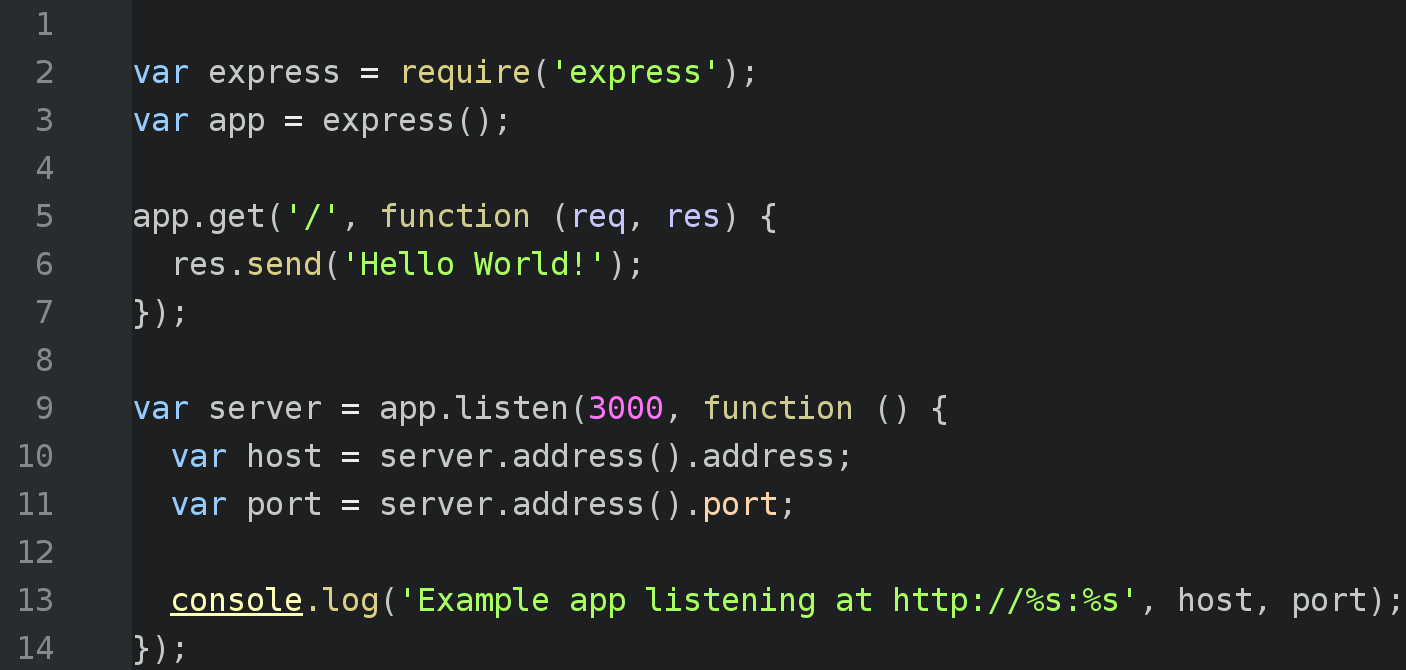
\includegraphics[scale=0.23]{assets/express_example.png}
\end{frame}

%----------------------

\section{Middleware/Frontend}

\begin{frame}
\Huge{
\centerline{Middleware/Frontend}
}
\end{frame}

%------------------------------------------------

\begin{frame}
\frametitle{jQuery}
\begin{itemize}
\item Framework zum Vereinfachen von JavaScript
\item wird hauptsächlich für Frontend eingesetzt
\item kann im low-scale Bereich als nützliche AJAX middleware benutzt werden
\end{itemize}
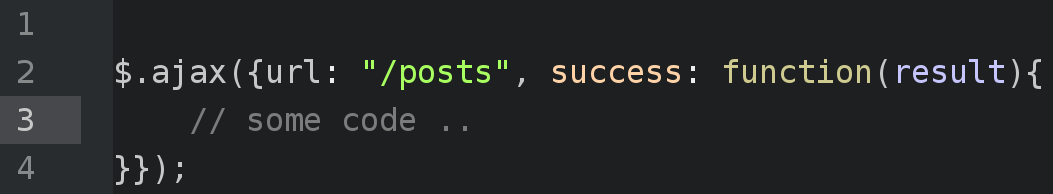
\includegraphics[scale=0.3]{assets/jQuery.png}
\end{frame}

%----------------------

\begin{frame}
\frametitle{reactJS}
\begin{itemize}
\item Frontend framework
\item benutzt als Datenfluss den \textit{one-way-data-flow}
\end{itemize}
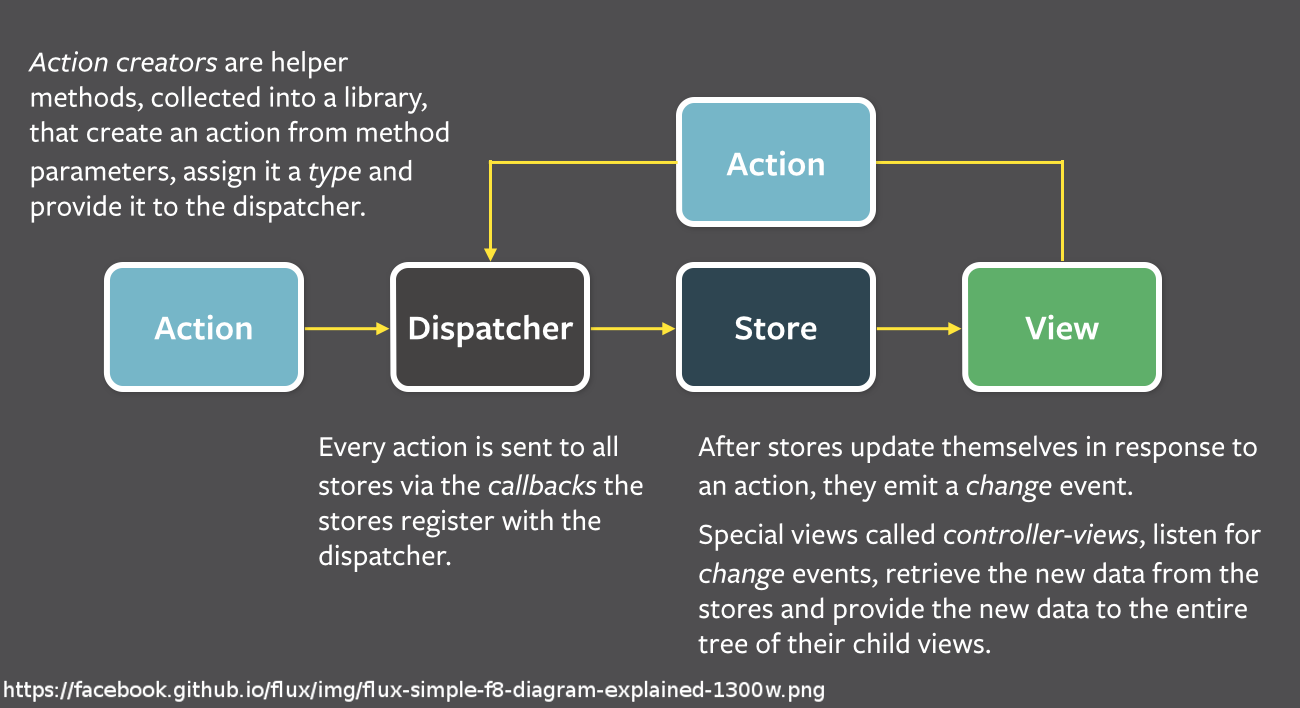
\includegraphics[scale=0.22]{assets/flux.png}

{\tiny https://facebook.github.io/react/img/blog/flux-diagram.png}
\end{frame}

%----------------------

\begin{frame}
\frametitle{angularJS}
\begin{itemize}
\item Frontend framework
\item benutzt als Datenfluss \textit{two-way-data-binding}
\end{itemize}
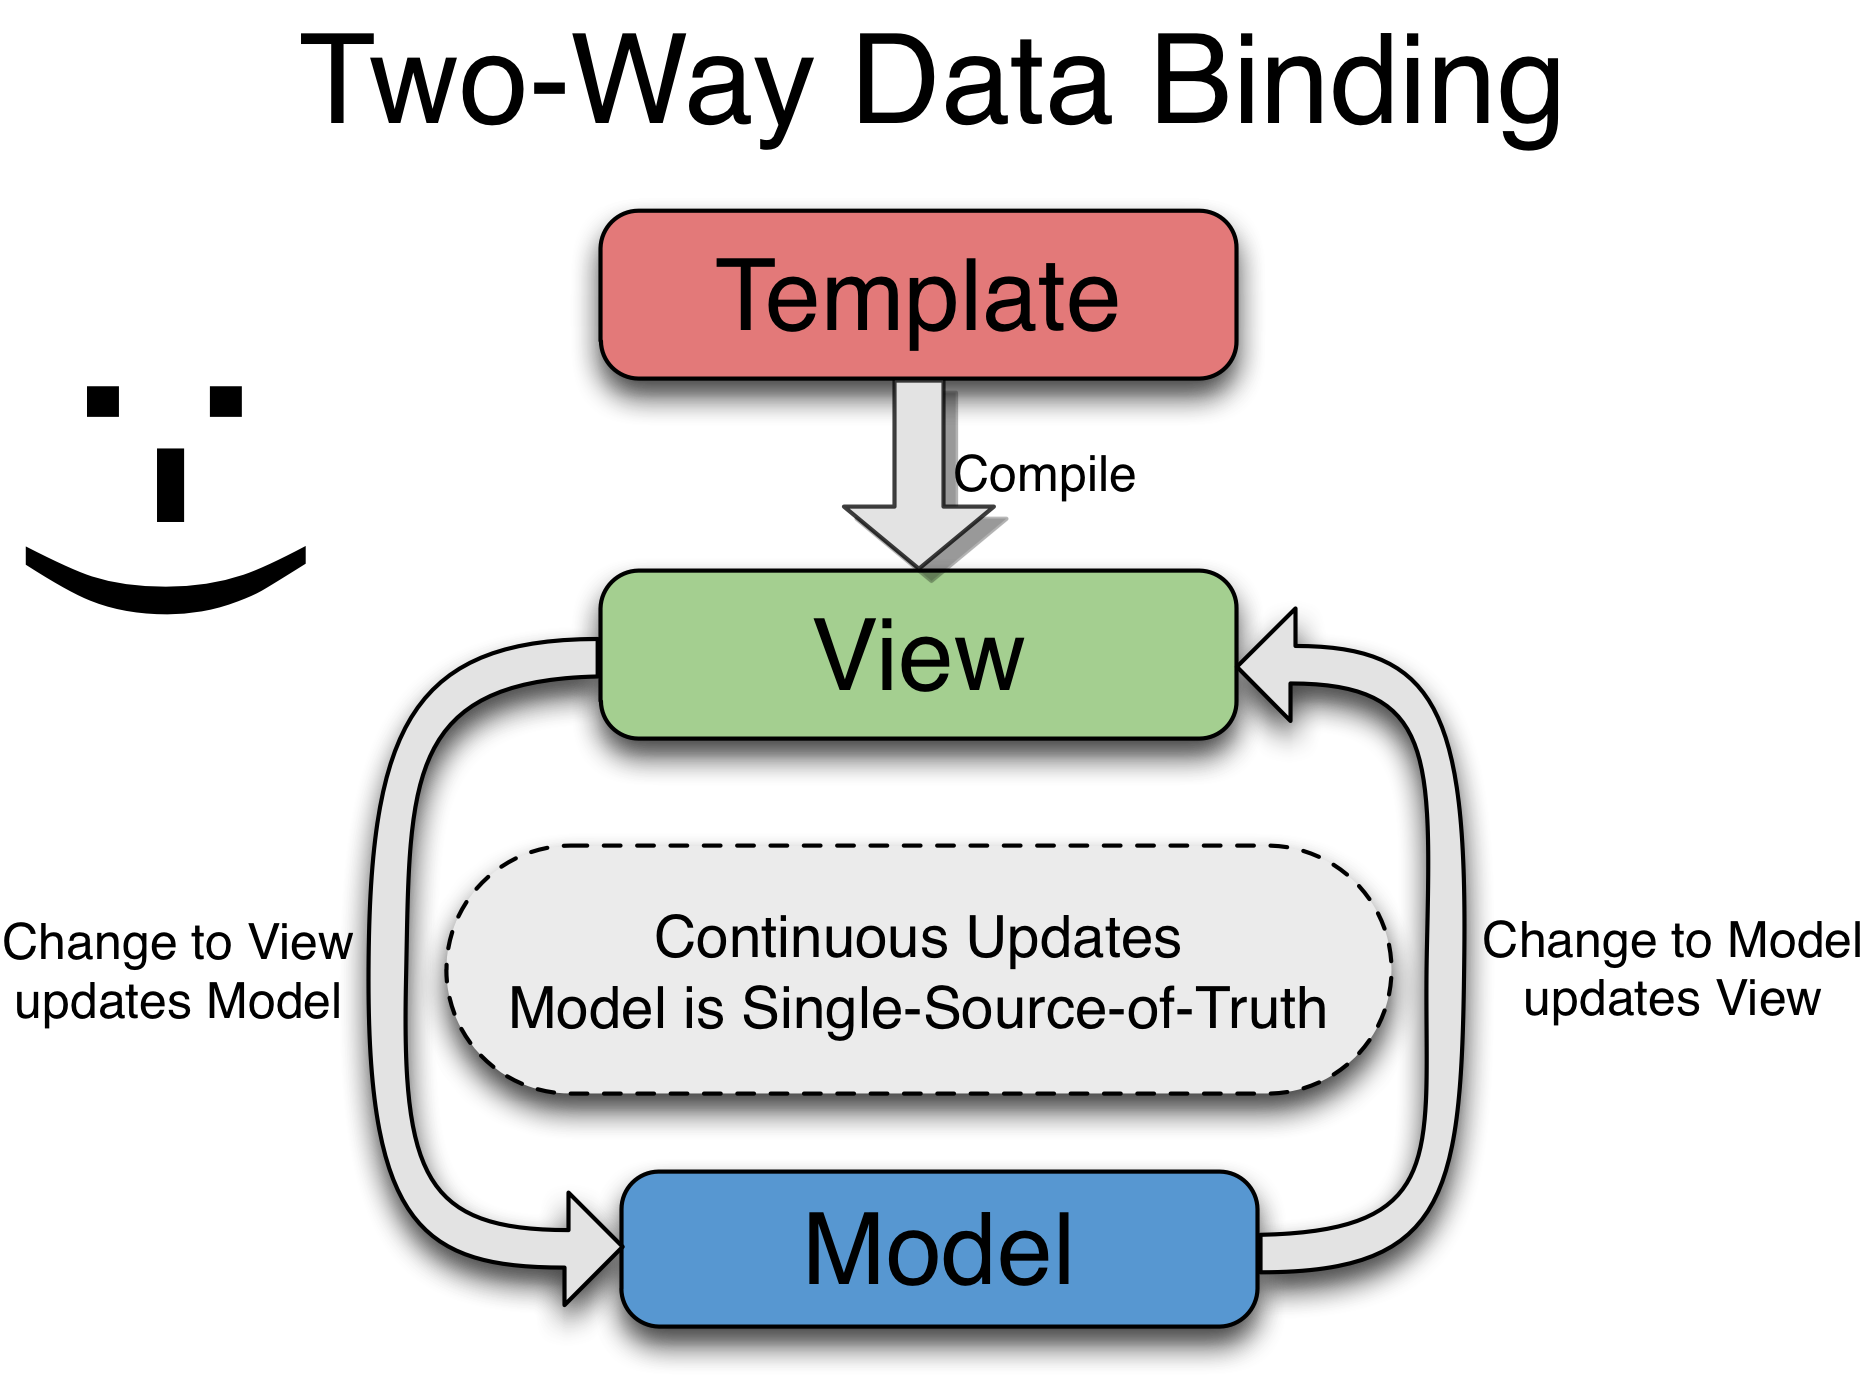
\includegraphics[scale=0.5]{assets/two-way-db.png}

{\tiny http://vojtajina.github.io/ng-slides/2011-09-23-web-expo/img/two-way-db.png}
\end{frame}

%----------------------

\section{Projektstruktur}

\begin{frame}
\Huge{
\centerline{Projektstruktur}
}
\end{frame}

%----------------------

\subsection{Dependency Management}

\begin{frame}
\Huge{
\centerline{Dependency Management}
\centerline{{\small Was ist das?}}
}
\end{frame}

%----------------------

\begin{frame}
\frametitle{Dependency Management: npm}
\begin{itemize}
\item für backend Applikationen
\item benutzt package.json datei für Abhängigkeiten
\item z.B.
\begin{itemize}
\item browserify
\item express
\item grunt
\item gulp
\item ...
\end{itemize}
\end{itemize}
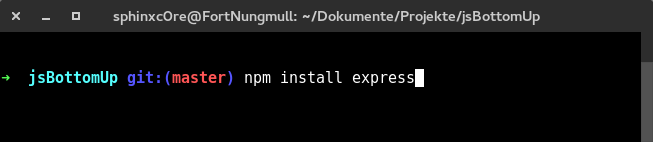
\includegraphics[scale=0.3]{assets/npm-cli.png}
\end{frame}

%----------------------

\begin{frame}
\frametitle{Dependency Management: bower}
\begin{itemize}
\item für frontend Applikationen (js, html, css, sass, coffescript, ...)
\item benutzt bower.json datei für Abhängigkeiten
\item z.B.
\begin{itemize}
\item jQuery
\item bootstrap
\item angular
\item react
\item ...
\end{itemize}
\end{itemize}
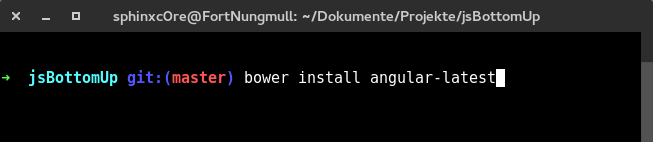
\includegraphics[scale=0.3]{assets/bower-cli.png}
\end{frame}

%----------------------

\subsection{Modularisierung}

\begin{frame}
\Huge{
\centerline{Modularisierung}
\centerline{{\small Was ist das?}}
}
\end{frame}

%----------------------

\subsection{Task Automatisierung}

\begin{frame}
\Huge{
\centerline{Task Automatisierung}
\centerline{{\small Was ist das?}}
}
\end{frame}

%----------------------






%------------------------------------------------
%--- THE END ------------------------------------

\begin{frame}
\Huge{\centerline{Danke für eure Aufmerksamkeit!}}

\begin{normalsize}

\centerline{\textit{pls clone https://github.com/SphinxC0re/jsBottomUp}}
\centerline{
\includegraphics[scale=0.2]{assets/like_button.png} 
\includegraphics[scale=0.2]{assets/dislike_button.png}}
\end{normalsize}
\end{frame}

%----------------------
\begin{frame}
\Huge{\centerline{Fragen? Anregungen?}}
\end{frame}

%----------------------



\end{document} 